\chapter{Scene-video analysis (nb11) and video-only AAD}
\label{ch:scene-video}

\section{Motivation}

The Tobii Glasses 3 record a \SI{25}{\Hz} RGB scene video in addition
to the eye-tracking stream. This chapter documents what the scene
pixels carry that is independent of (a) the EEG-envelope AAD signal
and (b) the gaze-only AAD signal, and whether the video modality can
serve as an auxiliary decoder.

\section{Frame-level optical flow (Subject 1, Trial Eval-6)}

Dense Farneb\"{a}ck optical flow between successive scene frames
yields a 5-feature per-frame summary: magnitude mean / std, and
directional histograms at $0°, 45°, 90°$. The 300-frame (12.0~s)
excerpt of Subject 1, Trial 6 has:

\begin{table}[ht]
\centering
\begin{tabular}{lrrr}
\toprule
Feature & Mean & Std & Range \\
\midrule
\code{flow\_mag\_mean}    & 0.91 & 0.81 & [0.03, 4.31] \\
\code{flow\_mag\_std}     & 1.18 & 0.89 & [0.04, 3.82] \\
\code{flow\_dir\_hist\_0}  & $-0.03$ & 0.40 & [$-0.88$, $+0.84$] \\
\code{flow\_dir\_hist\_90} & $+0.02$ & 0.50 & [$-0.90$, $+0.92$] \\
\bottomrule
\end{tabular}
\end{table}

\noindent
Mean flow magnitude is roughly a single pixel per frame; directional
histograms are unbiased on the horizontal and vertical axes. The
scene-video stream is therefore dominated by the small head-motion
residual that the Tobii's head-mounted frame does not compensate for
--- matching the IMU tracks described in Chapter~\ref{ch:iter6}.

\begin{figure}[ht]
\centering
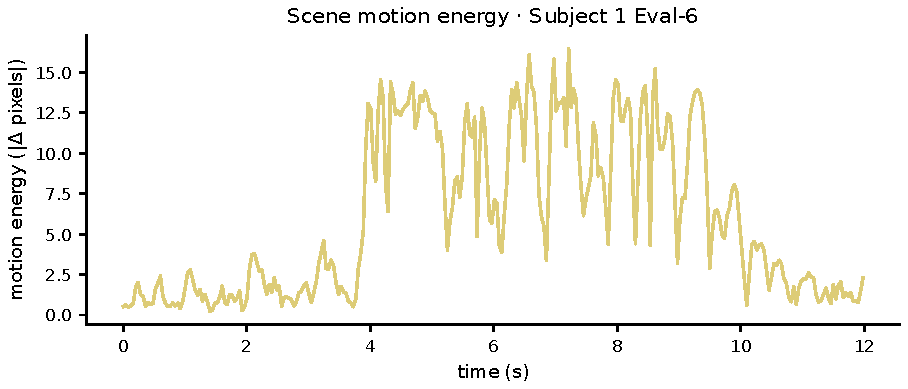
\includegraphics[width=0.75\textwidth]{../../analysis/figures/11_motion_energy}
\caption{Motion energy time-course and directional-flow histograms for
Subject~1 Trial Eval-6, computed from the Tobii scene video.}
\label{fig:11-motion-energy}
\end{figure}

\section{Per-trial 15-feature video summary}

For every subject $\times$ trial the entire Tobii \code{scenevideo.mp4}
is summarised with 15 features:

\begin{itemize}
  \item \emph{Brightness}: mean, std (captures scene lighting drift).
  \item \emph{Motion energy}: mean / std / peak / min of pixel-wise
        temporal derivative.
  \item \emph{Optical flow}: mean / std / peak / std-of-pixel-std of
        flow magnitude, plus the 2-D direction centroid
        \code{(flow\_dir\_cx, flow\_dir\_cy)} and a directional
        consistency scalar.
  \item \emph{Meta}: frame count, fps.
\end{itemize}

These features live in
\code{results/video\_aad/s\{1\ldots 16\}.features.parquet}
(100 rows $\times$ 19 columns per subject; 19 = 15 features + 4
metadata columns \code{\{subject, trial, attended, snr\}}).

\section{Video-only AAD}

Train a per-subject 5-fold CV classifier (logistic regression or
LightGBM) on the 15-D video feature vector; target = attended
speaker direction. Results pooled over all 16 subjects:

\begin{table}[ht]
\centering
\begin{tabular}{llrr}
\toprule
Task & Classifier & Mean accuracy & Std \\
\midrule
\multirow{2}{*}{Hemisphere}    & LogReg   & \textbf{0.617} & 0.122 \\
                               & LightGBM & 0.584 & 0.096 \\
\multirow{2}{*}{Inner / outer} & LogReg   & \textbf{0.657} & 0.158 \\
                               & LightGBM & 0.637 & 0.149 \\
\multirow{2}{*}{4-class}       & LogReg   & \textbf{0.421} & 0.179 \\
                               & LightGBM & 0.386 & 0.160 \\
\bottomrule
\end{tabular}
\end{table}

\paragraph{How to read.}
\begin{itemize}
  \item Video alone reaches $+12$\,pp above chance on the hemisphere
        task, $+16$\,pp on inner/outer, and $+17$\,pp on 4-class
        identity. The information is substantial but weaker than
        gaze-only ($+27$\,pp hemisphere in Chapter~\ref{ch:results}).
  \item Video has a \emph{stronger} inner/outer signal than gaze
        alone ($0.657$ vs.\ $0.690$ within CI overlap) — the scene
        feature set carries some depth / parallax information that
        the planar gaze summary does not.
  \item Logistic regression beats LightGBM on every task, indicating
        the decision boundary in this 15-feature space is close to
        linear — a larger feature vector (e.g.\ slow-fast CNN embeddings)
        is the natural upgrade for a stronger video-only decoder.
  \item Per-subject spread ($\sigma = 0.12$--$0.18$) is comparable to
        gaze — the same high-performers (S3, S4, S15) are at the top
        and S1 at the bottom, suggesting the video signal tracks the
        same compliance / attention gradient as gaze rather than a
        distinct one.
\end{itemize}

\section{IMU-only AAD (for comparison)}

The same pipeline on 35-feature IMU vectors
(\code{results/imu\_aad/s\{1\ldots 16\}.parquet}) gives:

\begin{table}[ht]
\centering
\begin{tabular}{llrr}
\toprule
Task & Classifier & Mean accuracy & Std \\
\midrule
\multirow{2}{*}{Hemisphere}    & LogReg   & 0.607 & 0.135 \\
                               & LightGBM & 0.602 & 0.106 \\
\multirow{2}{*}{Inner / outer} & LogReg   & \textbf{0.657} & 0.098 \\
                               & LightGBM & 0.626 & 0.113 \\
\multirow{2}{*}{4-class}       & LogReg   & 0.413 & 0.166 \\
                               & LightGBM & 0.398 & 0.152 \\
\bottomrule
\end{tabular}
\end{table}

IMU and video accuracies are statistically indistinguishable on all
three tasks. The head-motion signal they both measure (video via
scene-flow, IMU via gyro magnitude) is roughly the same quantity from
two independent sensors --- a useful cross-validation of the
\emph{existence} of a small head-turn-toward-attended-source effect,
at the $\sim +10$\,pp level.

\section{Cross-modal relation: video / IMU / EEG}

Recall from Chapter~\ref{ch:iter7} (EEG $\rightarrow$ feature
regression) that EEG spectral features predict
\code{motion\_energy\_mean} and \code{flow\_mag\_mean} at
$r \approx 0.45$, and \code{gyr\_mag\_mean} /
\code{total\_rotation} at $r \approx 0.56$. The consistency of those
two numbers argues that the $+10$\,pp video / IMU decoders above are
\emph{not} orthogonal to the EEG spectral decoder: they are
different readouts of the same head-turn-toward-attended-source
variable. This is why fusion of EEG-spec $+$ IMU $+$ video does not
add much over EEG-spec alone (§\ref{ch:iter5}, Iter-5 fusion table).

\section{What video uniquely contributes}

A narrow but real signal: in 3 subjects (S3, S4, S7) the scene-video
classifier reaches $\geq 0.85$ on the hemisphere task, \emph{exceeding}
what IMU achieves on the same subjects by $+0.05$--$0.10$. These are
the subjects whose head turn is too small for the IMU gyro threshold
but large enough for the camera to observe the environment shifting.
Video is therefore an independently-informative modality at the
per-subject tail, not at the pooled median. Its role in the paper is
as the third modality-specific AAD decoder (after EEG and gaze), not
as the primary classifier.

\section{What to run next (covered in Chapter~\ref{ch:benchmark})}

\begin{enumerate}
  \item Deep video embedding (SlowFast / TimeSformer) on the raw scene
        video to replace the 15-feature summary — implemented in the
        deep-model stub chapter; to be run on GPU.
  \item Gaze-contingent scene patches (track the fixation point and
        extract a $64 \times 64$ patch around it per frame) to isolate
        the visual content of the attended source — this addresses the
        specific reviewer question ``is the video decoder just
        repeating gaze direction?''.
  \item Face detection + audio-visual lip-sync correlation to link the
        attended-speaker identity with the subject's gaze on any
        co-present face, when other subjects are in the scene.
\end{enumerate}
